\def\layersep{1.4cm}

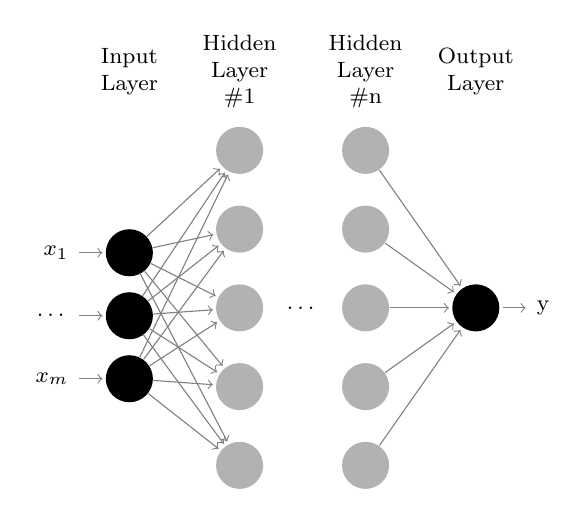
\begin{tikzpicture}[shorten >=1pt,->,draw=black!50, node distance=\layersep]
\footnotesize
    \tikzstyle{every pin edge}=[<-,shorten <=1pt]
    \tikzstyle{neuron}=[circle,fill=black!25,minimum size=17pt,inner sep=0pt]
    \tikzstyle{input neuron}=[neuron, fill=black!100];
    \tikzstyle{output neuron}=[neuron, fill=black!100];
    \tikzstyle{hidden neuron}=[neuron, fill=black!30];
    \tikzstyle{annot} = [text width=4em, text centered]

    % Draw the input layer nodes
    %\foreach \name / \y in {1,...,4}
    % This is the same as writing \foreach \name / \y in {1/1,2/2,3/3,4/4}
	
	\node[input neuron, pin=left:$x_1$] (I-1) at (0,-1.8) {};
	\node[input neuron, pin=left:\ldots] (I-2) at (0,-2.6) {};
	\node[input neuron, pin=left:$x_m$] (I-3) at (0,-3.4) {};


    % Draw the hidden layer nodes
    \foreach \name / \y in {1,...,5}
        \path[yshift=0.5cm]
            node[hidden neuron] (H1-\name) at (\layersep,-\y cm) {};


    % Connect every node in the input layer with every node in the
    % hidden layer.
    \foreach \source in {1,...,3}
        \foreach \dest in {1,...,5}
            \path (I-\source) edge (H1-\dest);
            
    % Dra second hidden layer nodes
    \foreach \name / \y in {1,...,5}
        \path[yshift=0.5cm]
            node[hidden neuron] (H2-\name) at (3.0,-\y cm) {};

    % Draw the output layer node
    %\node[output neuron,pin={[pin edge={->}]right:$y^{\inst_i}_1$}, right of=H2-2] (O-1) {};
    \node[output neuron, pin={[pin edge={->}]right:y}, right of=H2-3] (O-2) {};
    %\node[output neuron,pin={[pin edge={->}]right:$y^{\inst_i}_p$}, right of=H2-4] (O-3) {};

    % Connect every node in the hidden layer with the output layer
    \foreach \source in {1,...,5}
        \foreach \dest in {2,...,2}
            \path (H2-\source) edge (O-\dest);

    % Annotate the layers
    \node[annot,above of=H1-1, node distance=1cm] (hl1) {Hidden Layer \#1};
    \node[annot,right of=H1-3, node distance=.8cm] {\ldots};
    \node[annot,above of=H2-1, node distance=1cm] (hl2) {Hidden Layer \#n};
    \node[annot,left of=hl1] {Input Layer};
    \node[annot,right of=hl2] {Output Layer};
\end{tikzpicture}